\documentclass[journal,12pt,twocolumn]{IEEEtran}
\usepackage{graphicx}
\graphicspath{{./figs/}}{}
\usepackage{amsmath,amssymb,amsfonts,amsthm}
\newcommand{\myvec}[1]{\ensuremath{\begin{pmatrix}#1\end{pmatrix}}}
\usepackage{listings}
\usepackage{watermark}
\usepackage{titlesec}
\let\vec\mathbf

\titlespacing{\subsection}{0pt}{\parskip}{-3pt}
\titlespacing{\subsubsection}{0pt}{\parskip}{-\parskip}
\titlespacing{\paragraph}{0pt}{\parskip}{\parskip}
\newcommand{\figuremacro}[5]{
    
}
\lstset{
frame=single, 
breaklines=true,
columns=fullflexible
}
\thiswatermark{\centering \put(0,-105.0){
\includegraphics[scale=0.08]{logo.jpg}} }

\sloppy
\title{\mytitle}
\title{
Matrix Assignment - Conic
}
\author{T.Sai Raghavendra(FWC22087)}
\begin{document}
\maketitle
\tableofcontents
\bigskip


\section{\textbf{Problem}}
If the line x-1=0 is the directrix of the parabola to $y^2-kx+8=0$ then find one of the values of k
\begin{enumerate}
\item 4
\item $\frac{1}{4}$
\item 8
\item $\frac{1}{8}$
\end{enumerate}


\section{\textbf{Solution}}

we know that the vector equation of the line is 
\begin{align}
\label{eq:one}
\vec{n}^\top x = c
\end{align}

By comparing the given line with \eqref{eq:one} we get, 
\begin{center}
$\vec{n} = \myvec{1\\0}$ , c = 1 
\end{center}
We know that the equation of a conic with directrix $\vec{n}^\top x = c$, eccentricity e and focus F is given by 
\begin{align}
\label{eq:two}
\vec{x^\top Vx}+2\vec{u^\top}x+f = 0 
\end{align}
Compare the given parabola with \eqref{eq:two} we get,
\begin{center}
$\vec{V} = \myvec{0&0\\0&1}$ , $\vec{u} = \myvec{\frac{-k}{2} \\ \\ 0}$ , f = 8
\end{center}
Finding the vector $\vec{u}$ we can obtain the k value,\\ 
To find vector $\vec{u}$ we have,
\begin{align}
\label{eq:three}
\vec{u}=ce^2\vec{n}-||\vec{n}||^2\vec{F}
\end{align}
To find Focus $\vec{F}$ in \eqref{eq:three} we have,
\begin{align}
\label{eq:four}
f = ||\vec{n}||^2||\vec{F}||^2-c^2e^2
\end{align}
By substituting the f,c,e,$\vec{n}$ in \eqref{eq:four} we get,\\
\\$\vec{F} = 3\vec{e_1}$ $\implies$ $\vec{e_1} = \myvec{1 \\ 0}$ $\implies$ $\vec{F} = \myvec{3 \\ 0}$\\
By substituting the $\vec{F}$,c,e,$\vec{n}$ in \eqref{eq:three} we get,
\begin{center}
$\vec{u}$ = $\myvec{-2 \\ 0}$
\end{center}
Equating the vectors $\vec{u}$ we get,
\begin{center}
k = 4
\end{center}



\section{\textbf{Figure}}
\begin{figure}[h]
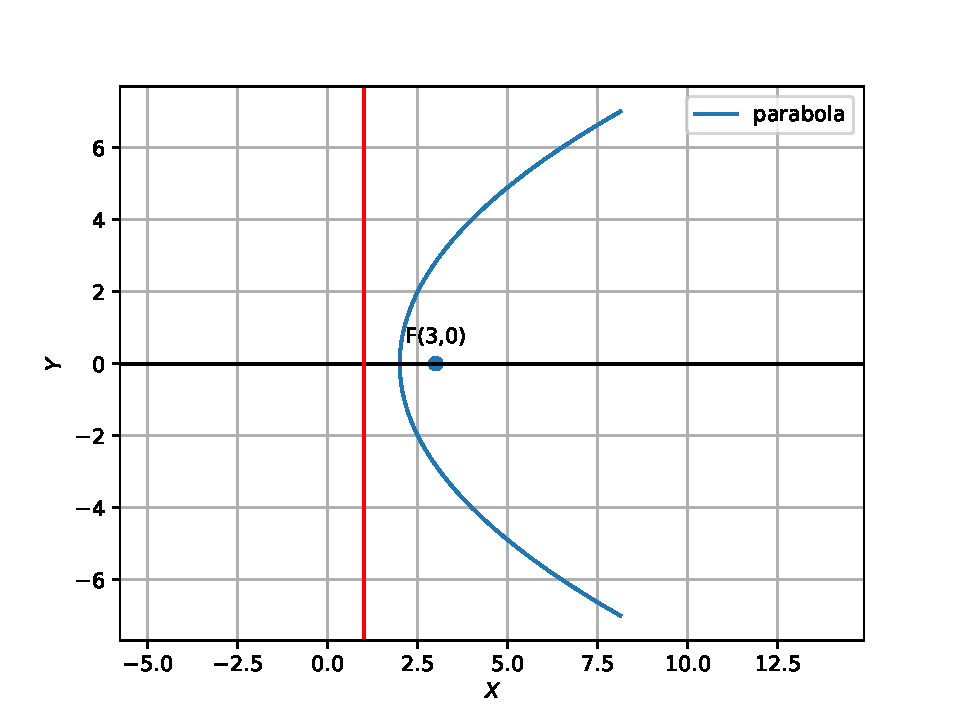
\includegraphics[width=\columnwidth]{fig.pdf}
\caption{To find the value of k and plotting the parabola}
    \label{fig:my_label}
\end{figure}


\begin{center}
$\vec{IV.\hspace{.2cm} Code Link}$
\end{center}
\begin{lstlisting}
https://github.com/Sairaghavendra36/Fwc-2022/blob/main/Matrices/Code/Conic.py
\end{lstlisting}
Execute the code by using the command
\textbf{python3 conic.py}


\end{document}